\documentclass{article}
\usepackage{newtxtext}
\usepackage[utf8]{inputenc}
\usepackage[legalpaper, left=1.40cm, right=1.40cm, top=0.95cm, bottom=2.54cm, a4paper]{geometry}
\usepackage[document]{ragged2e}
\usepackage{multicol}
\usepackage[T1]{fontenc}
\usepackage{setspace}
\usepackage{titlesec}
\usepackage{enumitem}
\usepackage{graphicx}
\usepackage[font=footnotesize]{caption}
\usepackage{etoolbox}

\usepackage{hyperref}

\patchcmd{\thebibliography}{\section*{\refname}}{}{}{}
\bibliographystyle{unsrt}
\captionsetup{justification=raggedright,singlelinecheck=false}
\graphicspath{ {./pic/} }
\makeatletter
\renewcommand{\fnum@figure}{Fig. \thefigure}
\makeatother



\font\myfont=cmr12 at 24pt
\setlength{\parskip}{6pt}
\renewcommand \thesection{\Roman{section}}
\titlespacing*{\section}{0ex}{0ex}{0ex}
\titleformat{\section}{\normalfont\normalsize\filcenter}{\thesection.}{1em}{}
\setlist[itemize,1]{leftmargin=0pt,itemindent=30pt, labelsep=10pt, parsep=0pt, topsep=1pt}
\setlist[enumerate,1]{leftmargin=0pt,itemindent=30pt, labelsep=10pt, parsep=0pt, topsep=1pt}
\renewcommand{\labelenumii}{\arabic{enumi}.\arabic{enumii}}

\begin{document}
  \begin{Center}
    {\myfont Algorithm for Detecting Anomalous Student\\Activities in the Online Learning Process Based on\\Box Plots\\}
  \end{Center}
  \bigbreak
\begin{multicols}{2}
  \begin{justify}
    \begin{Center}
      \begin{small}
        Liliya A. Demidova\\
        \textit{
          Institute for Information Technologies\\
          Federal State Budget Educational Institution of Higher Education\\\guillemotleft MIREA – Russian Technological University\guillemotright\\
        }
        Moscow, Russia\\
        liliya.demidova@rambler.ru\\
        Anastas A. Misailidi\\
        \textit{
          Institute for Information Technologies\\
          Federal State Budget Educational Institution of Higher Education\\\guillemotleft MIREA – Russian Technological University\guillemotright\\
        }
        Moscow, Russia\\
        misailidi.a@gmail.com\\
      \end{small}
    \end{Center}
  \end{justify}
\end{multicols}
\bigbreak
\begin{multicols}{2}
  \begin{justify}
    \begin{small}
      \textbf{
        \textit{Abstract}---The proposed research presents an algorithm for detecting anomalous student activities during online Python programming education, based on box plot analysis. Throughout their learning journey, students submit solutions to unique exercises across a range of tasks for assessment within the Digital Teacher Assistant (DTA) system. Anomalous activities are defined as those involving an excessively high number of solution submissions for a particular task or those characterized by extremely prolonged durations of task-solving. In both cases, students require timely assistance from instructors to clarify challenging course material. Upon each new submission of an exercise solution into the DTA system, the characteristics of the box plots for that specific task are recalculated. Decisions are made regarding whether the student's submission constitutes an anomaly (outlier), either in terms of the number of submissions or the duration of task-solving. The experimental results, using a dataset collected during the spring semester of 2023 at RTU MIREA, indicate the practical viability of implementing the proposed algorithm for the real-time detection of various anomalous activities (outliers) in students' interactions with the DTA system.
      }

      \textbf{
        \textit{Keywords---Anomalous activity, outlier, box plot, algorithm, Digital Teacher Assistant+}
      }
      \end{small}

      \section{INTRODUCTION}
      Today education is undergoing revolutionary changes thanks to modern technologies and innovations. One of the key components of this transformation is educational data analytics, which opens up unique opportunities for educational institutions and educators to improve the quality of learning and adapt to the needs of each student. Educational data analytics is a powerful tool in education, enabling the extraction of valuable insights from vast amounts of information collected during the learning process and using them to optimize teaching strategies, create personalized courses, and enhance the overall effectiveness of education.
      
      Educational Data Mining (EDM) is a field that focuses on applying data analysis methods to extract valuable knowledge and patterns in the educational environment. EDM utilizes various methods and techniques to analyze data collected from various educational sources such as e-textbooks, online courses, and learning platforms.

      As of the current moment, tracking underperforming students and the field of educational data mining remain pivotal in the realm of education. Modern technologies and analytical methods continue to play a crucial role in the analysis of vast datasets collected during online learning and courses \cite{1}. Presently, the primary focus is on identifying complex patterns and trends related to student performance, as well as providing individual recommendations to optimize the learning process. State-of-the-art algorithms are designed to proactively identify student challenges, enhance their motivation and engagement in learning, and reduce student attrition from educational programs \cite{2}. This area of scientific research continues to evolve actively, offering endless prospects for improving the quality of education and achieving greater efficiency in the field of education.

      In EDM, the following data analysis tools are considered.
      \begin{itemize}
        \item Cluster Analysis. This tool allows for the grouping of students into clusters based on their activity and learning performance. It can help identify different learning styles and student needs \cite{3}.
        \item Classification and Prediction. This tool enables the creation of models using machine learning algorithms to predict student success, identify outlier risks, or recommend individual learning paths.
        \item Association Rules. This tool helps discover relationships and dependencies between student actions in the educational environment.
        \item Factor Analysis. This tool helps uncover hidden factors influencing student success, such as motivation, preferences, and the educational environment.
        \item Text Data Mining. This tool is used for analyzing textual data, such as essays, reviews, and student comments, to identify trends and sentiments.
        \item Data Visualization. This tool allows educators and administrators to present information about students and educational processes in a more visual manner, aiding in making well-informed decisions \cite{2}.
        \item Data Analysis in Recommender Systems. This tool uses data analysis to provide students with course recommendations, materials, and learning strategies based on their previous experiences and interests \cite{5}.
        \item Graph Analytics. This tool enables the analysis of students' social networks and interactions within the educational environment.
      \end{itemize}

      These tools are used in EDM to optimize the educational process, improve learning outcomes, and create more personalized learning experiences for students \cite{6}.

      Massive online education, especially in the field of programming languages, is rapidly evolving. With the advent of online platforms and courses such as Coursera, edX, Codecademy, and many others, students and professionals worldwide have gained access to extensive libraries of educational resources, allowing them to learn programming languages at their own pace and at a convenient time. This has led to the democratization of education and increased accessibility of programming knowledge for everyone, regardless of their location and financial resources. Many of these courses offer interactive tasks, projects, and practical exercises, which contribute to a deeper understanding of programming languages and the enhancement of IT skills. Massive online education in the field of programming languages has truly transformed people's ability to learn and apply technological skills, making programming more accessible and inclusive for all \cite{7}.

      Timely identification of learners experiencing difficulties in mastering specific topics within a course is of significant interest, with the aim of enabling timely intervention by educators to address emerging issues, such as providing additional materials or explanations.
      
      \section{PROBLEM STATEMENT}
      The discipline “Python Programming” at RTU MIREA provides students with the opportunity to solve problems online on the corresponding website, demonstrating the modern direction of online education at its best. This discipline serves as a shining example of the convergence of modern technology and education, offering students a more interactive and practically oriented educational experience \cite{8}.

      Studying this discipline involves using DTA, which offers students unique exercises for various types of tasks. This enables students not only to study theory but also to immediately apply the acquired knowledge in practice. Interactive assignments and practical exercises, created in a digital environment, foster a deep understanding of the programming language and its application in real-life situations. Moreover, the online format allows students to learn at their convenience and pace, which is particularly important in today's fast-paced life.

      This discipline also exemplifies the principle of educational accessibility since it is accessible online and can be studied by students from different geographical regions, contributing to the global democratization of programming knowledge. Online resources of this kind provide unique opportunities for students, helping them develop sought-after skills in the field of information technology in an interactive and engaging manner.

      What makes DTA particularly valuable is that each problem variant is autogenerated. This means that students are provided with different versions of the same problem, ensuring the fairness and reliability of assessment. It also encourages students to approach problem-solving based on their understanding of the material rather than mechanical repetition of answers \cite{9}.

      When a student completes an exercise for a problem and submits their solution to the DTA system, it is automatically checked by the system for correctness. This ensures quick feedback and instant results. Furthermore, students' solutions are automatically clustered based on their approaches, further motivating students to explore all possible ways to solve a single problem. If a student successfully completes exercises for all 11 mandatory tasks, they have the opportunity to undergo intermediate assessment in the form of a credit, confirming their knowledge and skills in programming \cite{10}.

      Data collection and dataset creation based on learning outcomes are important steps that can provide valuable information for analysis and decision-making in the educational environment. This article analyzes a dataset containing information about the interactions of second-year students at RTU MIREA with the DTA system while studying the "Python Programming" course in the spring of 2023. The dataset examined in the proposed research includes the following columns \cite{11}.

      \begin{enumerate}
        \item Student Group: This column identifies the student's group affiliation. It can be valuable information for segmenting and analyzing student performance by groups.
        \item Problem Number: This column indicates the specific problem number that the student attempted to solve. It allows tracking which problems are more challenging and require additional support.
        \item Variant: Each problem has its own variant, allowing students to practice on different problems of the same type.
        \item	Date and Time of Submission: This column reflects the moment when the student submitted their problem solution. Analyzing the timing can help identify temporal trends in student activity.
        \item	Outcome: Here, the result obtained by the student for solving the problem is recorded. This is a key metric that can be used to assess student performance and the effectiveness of the educational process.
        \item	Student ID: A unique identifier for each student, enabling the analysis of individual student performance and activity.
        \item	Solution Method ID: This column may contain information about the method or strategy used by the student when solving the problem. It can be useful for analyzing different teaching methods and their impact on student outcomes.
      \end{enumerate}

      The dataset under consideration can be used for conducting various types of research, such as investigating successful teaching methods, studying identified patterns in student behavior, and researching factors influencing academic performance. Based on the results of such research, recommendation systems can be developed to enhance the educational process \cite{12}.

      For further analysis of this dataset and the identification of various types of student activities within it, the following features can be extracted.

      \begin{itemize}
        \item	Indicator of whether the student solved the task. This is a binary feature that indicates whether the student solved the task (True) or not (False).
        \item	Date of the student's task completion. This feature reflects the date when the student successfully completed the task. It can be used to analyze temporal trends in performance.
        \item	Date of the student's first attempt to solve the task. This feature indicates the date and time when the student first attempted to solve the task. It can help identify how quickly students start working on a task after it becomes accessible.
        \item	Duration from the task publication to its completion by the student. This feature shows how much time it took the student from the first attempt to successfully solve the task. This feature can help determine the difficulty level of tasks for students.
        \item	Number of tasks solved by the student on the first attempt. This feature allows identifying which students more frequently solve tasks on their first attempt, which may indicate their high competence.
        \item	Number of attempts by the student before successfully solving the task. This feature indicates the number of unsuccessful attempts made by the student before successfully solving the task. It can be an indicator of the student's effort and persistence.
        \item	Duration between the task publication and the student's first attempt to solve the task. This feature helps determine how quickly students respond to the appearance of new tasks and start working on them.
        \item	Number of different methods or approaches used by the student to solve the task. This feature indicates the number of different methods or approaches that the student used when solving the task. It can help identify diversity in students' approaches to problem-solving. 
      \end{itemize}

      Analyzing these features will help us better understand how students learn and solve exercises and tasks, identify successful teaching strategies for the discipline, factors influencing student success, and optimize the educational process to enhance its effectiveness \cite{13}.

      The examination of the dataset under consideration can be conducted in the context of addressing the following tasks to improve the quality of the educational process and optimize teacher resources.

      \begin{enumerate}
        \item	Providing Teacher Recommendations: This task involves creating a tool that automatically analyzes data on student performance and understanding of the course material. Based on this analysis, it provides recommendations to teachers regarding which topics to cover in their classes. Data analysis can be used to determine which topics and materials are best suited for specific groups of students. This will allow teachers to more accurately tailor their curriculum to the needs of specific student groups \cite{11}.
        \item	Notifying Teachers of Group Lagging: This task involves creating a notification system that automatically alerts teachers if a group of students starts falling behind or experiences difficulties in understanding the material. This enables teachers to promptly respond to challenges, addressing them before the next class and providing additional resources or support if necessary. It can also contribute to a more efficient use of class time.
        \item	Identifying Underperforming Students: This task involves developing a tool to identify underperforming students. Data analysis can be used to identify students with lower learning outcomes or difficulties in specific aspects of the course material. This allows teachers to pay special attention to underperforming students and provide them with personalized support and advice to improve their performance.
      \end{enumerate}
      The aim of this research is to identify real-time anomalous activities that describe students experiencing difficulties in learning specific topics of the “Python Programming” course by analyzing the number of unsuccessful attempts to solve exercise tasks and the amount of time spent on solving exercise tasks.
      \section{THEORETICAL PART}
      To achieve the stated goal in the proposed research, an iterative algorithm has been developed that operates on real-time data, allowing the analysis of student activity based on the time of uploading answers (solutions to exercises in 11 tasks) to the DTA system \cite{15}.

      The algorithm is based on calculating the characteristics of box plots using the outlier detection method with the interquartile range $IQR$ and can be described by the following sequence of steps.

      \begin{enumerate}
        \item Calculate the interquartile range $IQR$:
        $$IQR = Q3 - Q1,$$
        where $Q1$ is the first quartile (25th percentile) of the data, and Q3 is the third quartile (75th percentile) of the data.
        \item Calculate the upper bound (upper whisker) for outliers:
        $$Upper Boumd = Q3 + (1.5 * IQR),$$
        where 1.5 is the coefficient that determines which values are considered outliers. This coefficient can be adjusted depending on the data analysis requirements. Typically, a value of 1.5 is used, but in some cases, other values can be used to be more or less strict in identifying outliers.
        \item Determine the lower bound (lower whisker) Lower Bound for outliers:
        $$Lower Bound=Q1-(1.5*IQR).$$
        \item Consider the analyzed value as an outlier if it is less than the Lower Bound or greater than the Upper Bound.
      \end{enumerate}
      
      The algorithm follows a standard approach to detect outliers in the analyzed dataset, based on calculating interquartile ranges for feature values. In particular, it calculates the interquartile ranges for the feature values describing the number of unsuccessful attempts by a specific student in solving a specific task and for the feature values representing the duration of solving a specific task by a particular student. This calculation is done each time a new solution for a task by a student is uploaded.

      The proposed algorithm can be described by the following sequence of steps.
      \begin{enumerate}
        \item Sort the records of uploaded responses by time (in ascending order).
        \item Create an empty table called ”Successful Uploads”.
        \item Create an empty list called “Analyzing Records”.
        \item Create an empty list called “Outlier Students by Number of Attempts”.
        \item Create an empty list called “Outlier Students by Solution Duration”.
        \item Create a dictionary called “Bounds of Boxplots by Number of Attempts” with pairs where the key is the task number, and the value is an empty list.
        \item Create a dictionary called “Bounds of Boxplots by Solution Duration” with pairs where the key is the task number, and the value is an empty list.
        \item For each record in the sorted data:
        \begin{enumerate}[leftmargin=-2pt, itemindent=37pt]
          \item If the student successfully solves the task:
          \begin{itemize}[leftmargin=30pt, itemindent=0pt]
            \item Add a record to the “Successful uploads” table.
            \item	Finish the iteration of the loop.
          \end{itemize}
          \item If the task is solved incorrectly, and there is no record of a previous successful solution to this task:
          \begin{itemize}[leftmargin=30pt, itemindent=0pt]
            \item Add a record to the “Analyzing Records” list.
            \item Generate a table from rows based on the current task.
            \item Group the “Table from Rows by Current Task” by students.
            \item Count the number of unsuccessful attempts to solve the task for each student by counting the rows in the subtables.
            \item Calculate the time from the publication of the task to the moment of the student's last submitted solution.
            \item Calculate the current boxplot boundaries based on data on the number of uploads by all students, including the 25\% (Q1) and 75\% (Q3) quartiles, median, left, and right whiskers.
            \item Add the obtained values to the list obtained by the current task number from the “Boxplot Boundaries by Number of Attempts” dictionary.
            \item Calculate the current boxplot boundaries based on data on the time spent on solving all students, including the 25\% (Q1) and 75\% (Q3) quartiles, median, left, and right whiskers.
            \item Add the obtained values to the list obtained by the current task number from the “Boxplot Boundaries by Duration of Solution” dictionary.
            \item Find students who are outliers in the number of incorrect submissions for the current task.
            \item Find students who are outliers in the duration of solving the current task.
            \item Replace old rows in the “Students Outliers by Number of Attempts” list related to the current task with new ones.
            \item Replace old rows in the “Students Outliers by Duration of Solution” list related to the current task with new ones.
            \item When new data is received, it is possible to run a single iteration of the loop without restarting the entire loop and update the statistics without restarting the algorithm from the beginning.
          \end{itemize}
        \end{enumerate}
      \end{enumerate}
    \end{justify}
  \end{multicols}

  \begin{figure}[h]
    \centering
    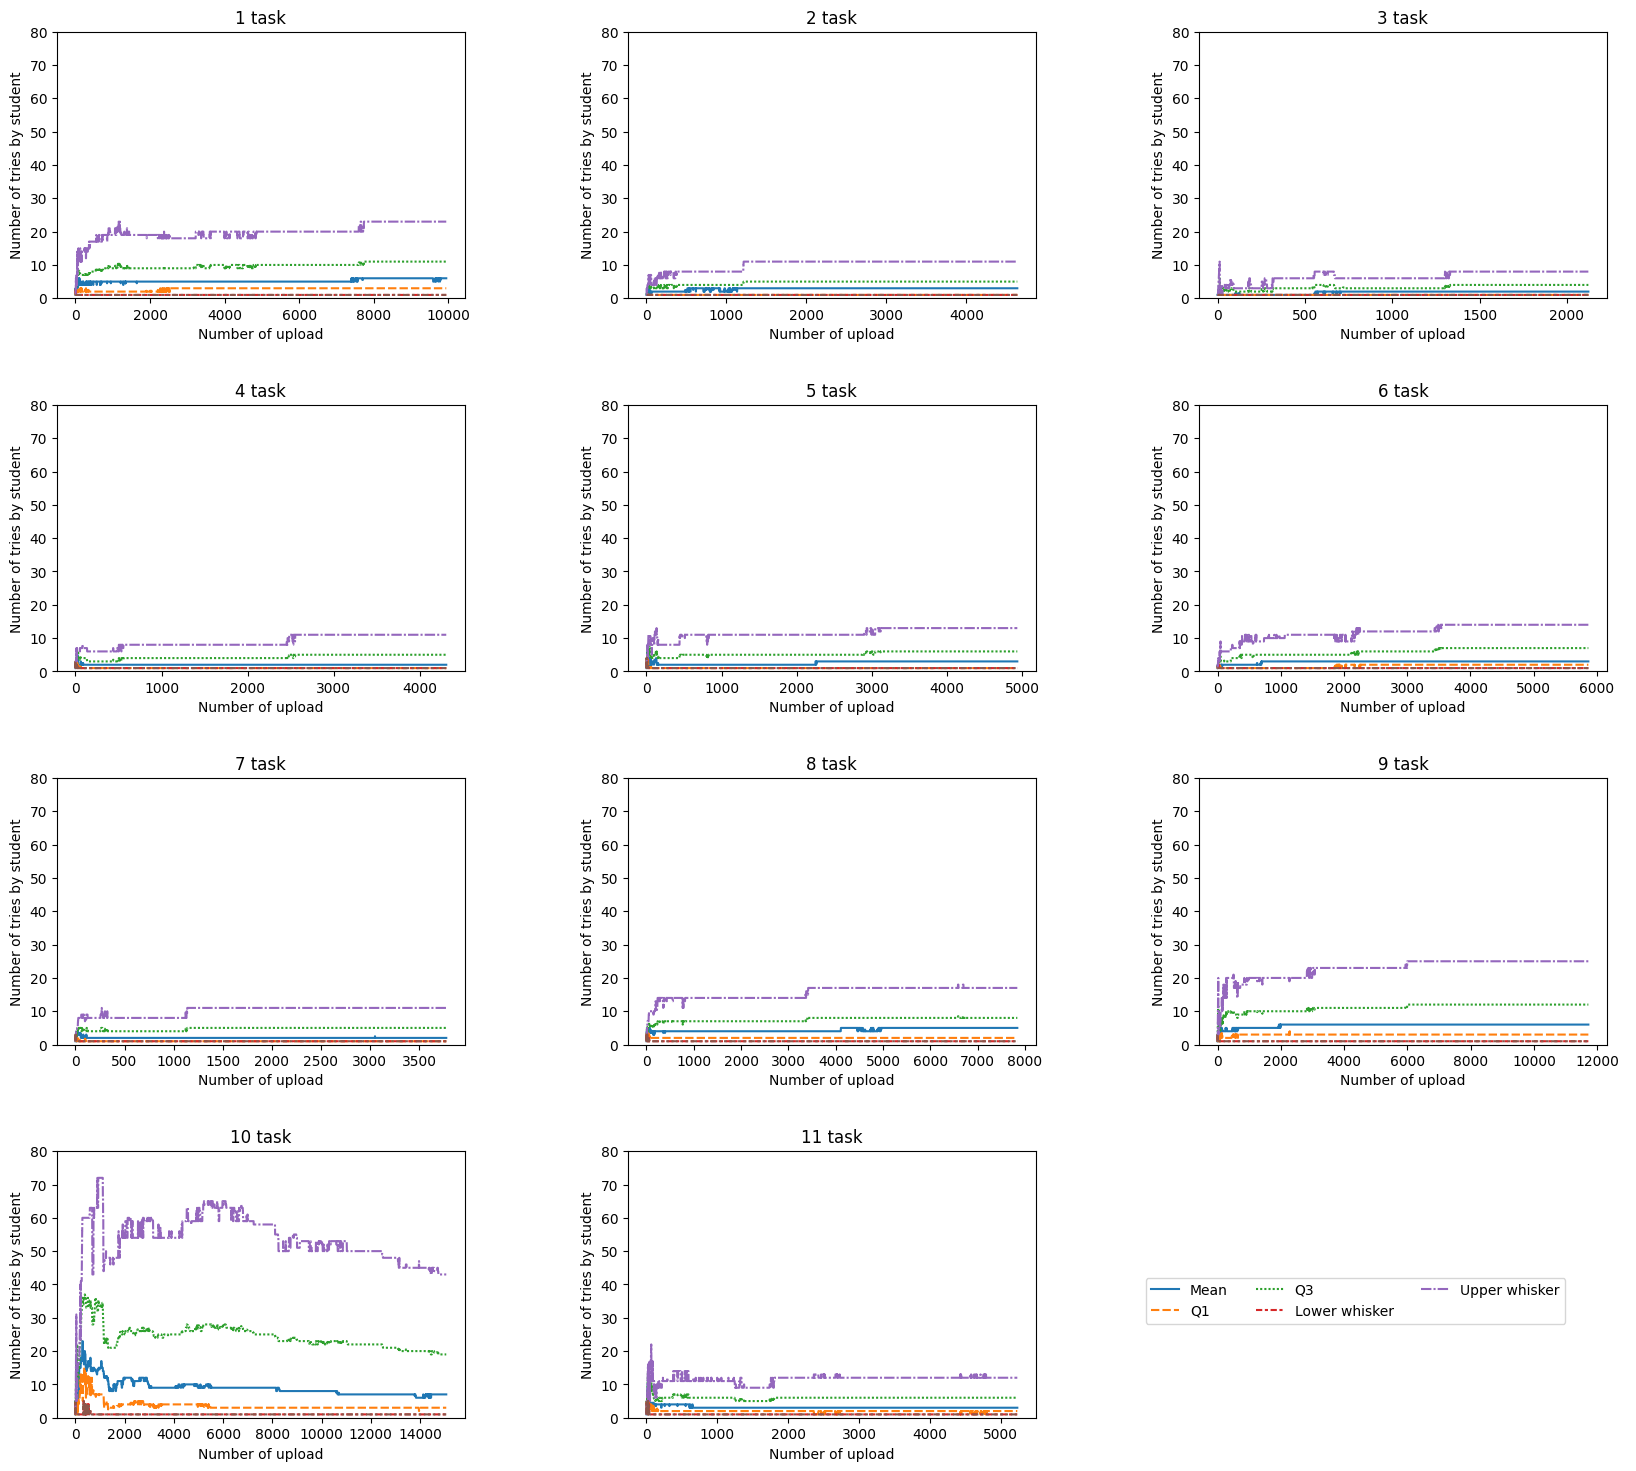
\includegraphics[width=\linewidth]{pic1.png}
    \caption{Graphical dependencies based on box plots of the number of solution uploads for tasks}
    \label{fig:pic1}
  \end{figure}
  \begin{figure}[h]
    \centering
    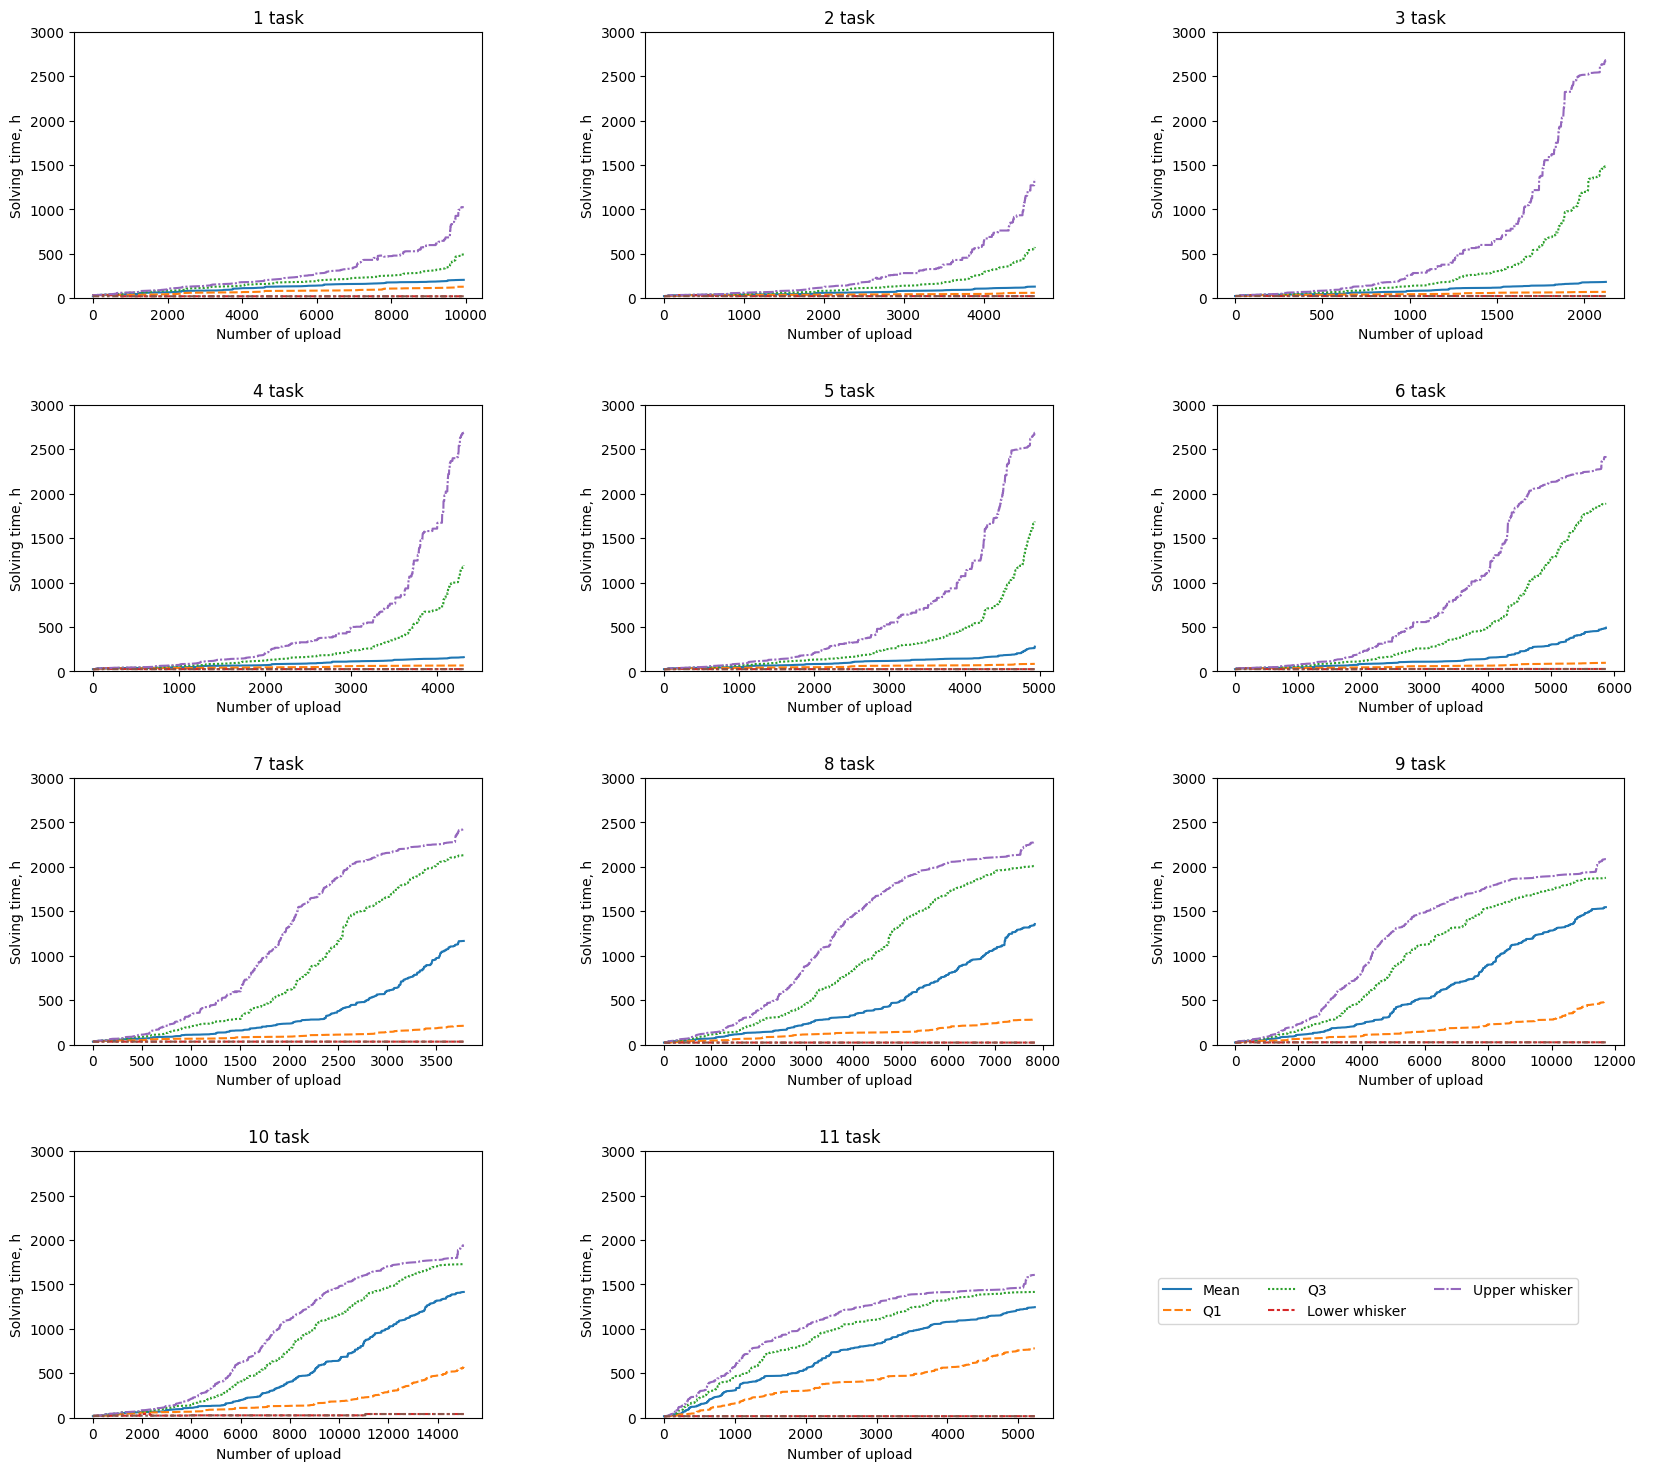
\includegraphics[width=\linewidth]{pic2.png}
    \caption{Graphical dependencies based on box plots of the duration of task solutions}
    \label{fig:pic2}
  \end{figure}

  \begin{multicols}{2}
    \begin{justify}
      \section{EXPERIMENTAL PART}
      The software implementation of the proposed algorithm was done using Python 3.10 in the Google Colab environment.

      The search for abnormal student activities was carried out in the context of solving the problem of detecting students who have difficulties in solving exercises on various tasks. Accordingly, for each task, monitoring of successful and unsuccessful solution uploads of exercises was performed.

      Figures \ref{fig:pic1} and \ref{fig:pic2} depict graphical dependencies for each task obtained as a result of applying the proposed algorithm, which is based on the analysis of box plots. This analysis is performed after each upload of a task solution to the DTA system. The figures display changes in the boundaries of the box plot for the number of incorrect solutions (Figure \ref{fig:pic1}) and the duration of solutions (Figure \ref{fig:pic2}) depending on the receipt of new data.

      The blue line in each figure represents a graphical dependency based on the median values of the number of solution uploads (duration of solution) for the task at the time of each upload. This graphical dependency is smoother than other dependencies based on Q1, Q3, as well as the boundary values for the lower and upper whiskers of the box plot. This is because these parameters are formed based on the results of accumulating a certain number of records and determining whether certain students have become outliers or have ceased to be.

      In Figure \ref{fig:pic1}, the graphical dependencies in all subfigures, except for the one corresponding to the 10th task, show that the average number of uploads is increasing. This is due to the fact that the 10th task is more complex, so it is characterized by many outlier students and a much larger spread of the whisker values compared to other tasks. At each moment when a student uploads a solution to a specific task, it is checked whether this upload of a specific student is an outlier or not. Then, the median, Q1, Q3 values, as well as the boundary values for the lower and upper whiskers of the box plot, are recalculated, taking into account this information for further monitoring and the construction of graphical dependencies for making certain pedagogical decisions.

      In addition to the number of attempts to solve a task by a student, the duration between the publication of the task and its successful solution can also be analyzed.

      Analyzing the duration is an important aspect when studying student activity in an educational environment. A long-time interval between the publication of a task and its successful solution may indicate a student's weak theoretical preparation and difficulties in assimilating the study material. This indicator can help teachers identify students who require additional assistance and support for successful learning \cite{16}.

      The growth rate of the graphs may be related to the number of submissions and the complexity of the task. The more complex the task, the longer it takes to solve, and the greater the number of submissions required for a solution.

      The smoother the graph, the more submissions each student makes. If a task is simple, students solve it with a small number of attempts, but many students postpone solving simple tasks until the last moment. As a result, simple tasks show a steep growth in the graph.

      A large number of motivated students solved the first task quickly and without any problems, so the graph is closely aligned with the x-axis. In the case of the third task, there are no difficulties either, but a significantly smaller number of students solve it, resulting in a relatively small number of submissions, but the graphs start growing quickly. In the tenth task, there are a huge number of attempts, but they are made by a smaller number of students, so they are close in time to each other, resulting in a smoother growth of the graph.

      Students who fall below the median value, on average, solve tasks more quickly than others and require fewer attempts to do so. Their activity can also be tracked through analysis and encouraged.

      The values on Figures \ref{fig:pic1} and \ref{fig:pic2} that fall above the purple line or below the red line are outliers. With the introduction of new data, some old data points may become outliers, and conversely, old outliers may cease to be outliers. As a result, graphical dependencies visualizing the boundary values of the upper and lower whiskers may fluctuate in both directions. The blue line represents the median value of the analyzed variable, and it is used as the central value rather than the mean because the median is robust to outliers. It is also worth noting that 50% of the sample falls between the graphical dependencies for the first and third quartiles, indicating where a significant portion of the data lies.

      \section{CONCLUSION}
      The proposed algorithm allows real-time analysis of statistics for each task and identifies changes in student performance, which can be a valuable tool for adapting the educational process and providing individual support to students. It will detect both students experiencing difficulties in the learning process and students who can easily solve even the most challenging tasks with a small number of submissions and in a short time.

      The goal of further work is to create an integrated system for analyzing student activity with the aim of providing recommendations to teachers, notifying teachers of groups of students falling behind, identifying struggling students, and tracking dishonest students. This system will be based on the analysis of student performance, activity, and understanding of the study material. It will enable teachers to more accurately adapt the educational process to the needs of students and respond promptly to emerging difficulties. Ultimately, it will lead to more efficient use of instructional time and an increase in student performance. 

      \section*{REFERENCES}
      \begin{footnotesize}
        \bibliography{paper.bib}
      \end{footnotesize}

    \end{justify}
  \end{multicols}      
\end{document}
